%!TEX program = xelatex
\documentclass[11pt,numbers=noenddot]{scrartcl}
\usepackage[ngerman]{babel}
\usepackage[a4paper,lmargin={2.5cm},rmargin={3.5cm}, tmargin={2.5cm},bmargin = {2.5cm}]{geometry}
\usepackage{amsmath}
\usepackage{mathabx}
\usepackage{mathtools}
\usepackage{stmaryrd}
\usepackage{enumitem}
\usepackage{graphicx}
\usepackage{courier}

\usepackage{relsize}
% \linespread{1.2}
\usepackage{setspace}
\onehalfspacing
% \usepackage[square]{natbib}
\usepackage{jurabib}
% \usepackage {algorithm2e}

% Package, das die Benutzung von Old Standard erlaubt
\usepackage{fontspec}

\setmainfont{OldStandard-Regular.otf}[
Path = /usr/local/texlive/texmf-local/opentype/,
BoldFont = OldStandard-Bold.otf,
ItalicFont = OldStandard-Italic.otf]

\bibliographystyle{jurabib}
\renewcommand*{\bibbtsep}{In: }
\renewcommand*{\bibjtsep}{In: }
\jurabibsetup{
  % authorformat=and,
  authorformat=italic,
}

% \makeatletter
% % \renewcommand{\l@section}{\@dottedtocline{1}{1.5em}{2.6em}}
% \renewcommand{\l@subsection}{\@dottedtocline{2}{4.0em}{3.6em}}
% \renewcommand{\l@subsubsection}{\@dottedtocline{3}{7.4em}{4.5em}}
% \makeatother

% \addtokomafont{disposition}{\normalfont}
\addtokomafont{sectionentry}{\normalfont\bfseries}


\setkomafont{subject}{\normalfont\small}
\addtokomafont{title}{\normalfont\bfseries}
\addtokomafont{section}{\normalfont\centering\bfseries}
\addtokomafont{subsection}{\normalfont\centering\bfseries}
\addtokomafont{subsubsection}{\normalfont\centering\bfseries}

\addtokomafont{publishers}{\normalfont\small}
\addtokomafont{date}{\normalfont\small}
\addtokomafont{author}{\normalfont\small}
\addtokomafont{descriptionlabel}{\normalfont\bfseries}

% \renewcommand{\thesection}{\Roman{section}} 
% \renewcommand{\thesubsection}{\thesection.\Roman{subsection}}


\subject{  Universität zu Köln \\
  Sprachliche Informationsverarbeitung \\
  Hauptseminar: Angewandte linguistische Datenverarbeitung \\
  Prof. Dr. Jürgen Rolshoven \\
  Hausarbeit
  }
\title{Semantische Spezifität \\im Word Space Model}
\author{Von C. Friedrich}
\date{(Vorgelegt am \today)}


\usepackage{amsthm}
\newtheorem*{defi}{Definition}


\begin{document}
\begin{titlepage}
\maketitle

\abstract{\textbf{Zusammenfassung.} In dieser Arbeit versuche ich experimentell zu bestätigen, dass Anglizismen im Deutschen semantisch spezifischer sind als ihre englischen Ursprungswörter. Dazu entwickle ich zunächst verschiedene Verfahren, die statistische Eigenschaften der Wörter im Deutschen und Englischen untersuchen und Rückschlüsse auf die semantische Spezifität zulassen sollen. Zentral ist dabei die Idee, dass spezifischere Wörter einen dichteren Kontext haben, analog zu der Dichte eines Clusters im Wortraum. Die entwickelten Verfahren werden anschließend empirisch überprüft.

Im nächsten Schritt wende ich diese Verfahren auf die zentrale These an. Dabei zeigen sich vielversprechende Resultate, die sich jedoch als noch etwas unausgereift erweisen. Daher wird die zentrale These nicht einheitlich experimentell bestätigt, die Ergebnisse indizieren jedoch das Potential der vorgestellten Maße.}

\thispagestyle{empty}
\end{titlepage}

\tableofcontents
\newpage

\section{Einleitung}

In dieser Arbeit verfolge ich zwei Ziele: Zum einen suche ich ein Maß für die semantische Spezifität von Worten. Dazu entwerfe ich, ausgehend von einigen Hypothesen, verschiedene Maße und teste diese dann mit Hilfe von Korpora und einem Testsatz von Wortpaaren. Zum anderen wende ich die so erprobten Maße auf die Fragestellung an, wie sich Anglizismen im Deutschen hinsichtlich ihrer semantischen Spezifität von ihren englischen Ursprungswörtern unterschieden. In Kapitel 2 und 3 beschäftige ich mich mit dem ersten Ziel, die Anwendung erfolgt in Kapitel 4. Ausgehend von folgenden drei Thesen stelle ich drei Maße für die semantische Spezifität vor:
\begin{enumerate}
    \item Spezifischere Wörter treten seltener auf.
    \item Spezifischere Wörter stehen mit weniger verschiedenen Wörtern im Kontext.
    \item Spezifischere Wörter verfügen über einen Kontext, der sich semantisch ähnlicher ist.
\end{enumerate}

These 1 tritt in dieser Arbeit in Form des \emph{Document Frequency Score} auf (siehe Abschnitt \ref{df}), These 2 in Form des \emph{Non-Zero Dimensions Score} (Abschnitt \ref{nzds}) und These 3 in Form des \emph{Mean Distance to Centroid Score} (Abschnitt \ref{mdcs}).

Die verwendeten Maße sind dabei statistische Maße, also Maße, die irgendetwas mit Zählen zu tun haben \citep[S. 4]{manning1999}. Konkreter: Maße, die sich auf die Anzahl bestimmter Eigenschaften von Wörtern in Texten beziehen. Welche Berechnungen man anschließend mit den gezählten Werten anstellt, legt das mathematische Modell fest. Ich werde dazu das \emph{Word Space Model} verwenden, das in Abschnitt \ref{wsm} vorgestellt wird.

\subsection*{Semantische Spezifität}
Was ist eigentlich semantische Spezifität? \citet[S. 11]{sparckjones1972} beschreibt die Spezifität eines Begriffes so:
\begin{quote}
  Specificity ... is a semantic property of index terms: a term is more or less specific as its meaning is more or less detailed and precise.
\end{quote}

Ein Wort hat also eine spezifischere Bedeutung, wenn es konkreter, detaillierter oder präziser ist. Ich denke, dass man so schnell ein intuitives Verständnis davon hat, was mit semantischer Spezifität gemeint ist. Anders formuliert ist ein Wort spezifischer, wenn es sich auf weniger Situationen anwenden lässt. Es schließt mehr Sachverhalte aus. Bezogen etwa auf die Tierwelt haben spezifischere Bezeichnungen eine geringere Extension: Mit 'Säugetier' kann man tausende verschiedene Tiere und Tierarten bezeichnen, mit 'europäischer Feldhamster' meine ich eine sehr spezielle Art von Tier.

Mit diesem intuitiven Verständnis von Spezifität wird auch schnell klar, wieso der Kontext des Wortes ein Indikator für dessen Spezifität sein kann. Ein spezifisches Fachwort tritt vorrangig zusammen mit anderen Wörtern aus dem selben Themenbereich auf, der Kontext ist eher eng gefasst. Ein allgemeines, vielseitig anwendbares Wort tritt mit allen möglichen Wörtern zusammen auf. Der Kontext ist sehr weit. Auch \citet{weeds-weir-mccarthy} stellen fest, dass generelle Worte eher in einem weiten Kontext auftreten als Spezifischere.

Diese naheliegende Idee versuche ich vorliegender Arbeit in ein mathematisches Modell zu übersetzen.

\subsection*{Semantische Spezifität und Anglizismen}

Ein Anglizismus ist ein Wort im Deutschen, das einen Ursprung im Englischen hat. \citet[S. 38]{schütte1996schöne} definiert so:

\begin{quote}
    Ein Anglizismus ist ein sprachliches Zeichen, das ganz oder teilweise aus englischen Morphemen besteht, unabhängig davon, ob es mit einer im englischen Sprachgebrauch üblichen Bedeutung verbunden ist oder nicht.
\end{quote}

\noindent \citet[S. 216]{burmasova2010empirische} fasst den Begriff etwas weiter:
\begin{quote}
    Alle sprachlichen Zeichen, deren englische Herkunft an der Form oder Semantik zu erkennen ist, gehören zu den Anglizismen.
\end{quote}

Weiter werden in der Literatur über verschiedene Paradigmen Kategorisierungsvorschläge gemacht, um den Begriff Anglizismus genauer zu bestimmen. Für meine Zwecke sind die Definitionen oben aber bereits ausreichend: Worte im Deutschen, die eine erkennbare englische Herkunft haben. Um Deutsch und Englisch miteinander zu vergleichen, muss allerdings eine eine-zu-eins-Zuordenbarkeit bestehen.

Wie verhalten sich nun Anglizismen und ihre englischen Ursprungswörter in Bezug auf ihre semantische Spezifität? Findet eine Bedeutungsverschiebung statt? Ich stelle in dieser Arbeit die These auf, dass Anglizismen in ihrer Verwendung im Deutschen dazu tendieren, \textbf{spezieller} zu sein als ihre englischen Ursprungswörter.

Für diese These argumentiere ich hier nicht traditionell sprachwissenschaftlich oder versuche sie zu erklären, sondern versuche lediglich, gemäß der statistischen Eigenschaften zu bestätigen, dass es sich tatsächlich so verhält.
% \newpage
\section{Ein Maß für die semantische Spezifität}

Das Maß für die semantische Spezifität soll in der Lage sein, von zwei Wörtern das semantisch Spezifischere herauszusuchen.

Für die Auswahl eines passendes \emph{Word Space Models} gibt es verschiedene Optionen. Im Information Retrieval weit verbreitet ist etwa eine Dokument-Wort-Matrix, in der für jedes Dokument des Korpus angegeben wird, wie häufig jedes analysierte Wort des Korpus darin auftritt. Eine solche vollständige Matrix ist eine Darstellung des sogenannten Dokumentenraums (\emph{Document Space}) \citep[S.296]{manning1999}. Ebenfalls weit verbreitet ist eine Wort-Wort-Matrix, die die Relationen der Wörter im Korpus untereinander einzufangen versucht. Sie stellt den sogenannten Wortraum dar (\emph{Word Space}). Ich werde mich ihn dieser Arbeit statt auf den Dokumentenraum vorrangig auf Methoden aus dem Wortraum stützen. \citet{Schutze:1994:CTT:2856823.2856847} argumentieren dafür, dass sowohl quantitativ als auch qualitativ reichhaltigere semantische Informationen auf Basis des \emph{Word Space Models} gewonnen werden können.

Wie die Relationen zwischen Wörtern aussehen können und wie man mit ihnen eine Näherung der semantischen Spezifität berechnen kann, möchte ich in diesem Kapitel vorstellen. Dazu entwickele ich verschiedene Berechnungsmethoden und kombiniere diese erst einmal ohne starke theoretische Vorannahmen. Dann stelle ich ein Experiment vor, dass die Berechnungsmethoden auf ihre Tauglichkeit zur Berechnung der semantischen Spezifität hin prüft. Die vielversprechendsten Methoden wende ich dann im anschließenden Kapitel auf die Fragestellung der semantischen Spezifität von Anglizismen an.

\subsection{Score 1: Document Frequency} \label{df}
Bereits \citet{sparckjones1972} schlug ein statistisches Maß für die semantische Spezifität eines Wortes vor. Es ist die simple Anzahl, mit der ein Wort im Korpus auftaucht, das ein Indiz für die Spezifität darstellen soll. \citet{Caraballo99determiningthe} konnten die \emph{Document Frequency} als Eigenschaft von Worten dazu nutzen, für beliebige Wortpaare festzustellen, welches Wort  spezifischer oder genereller ist. Überprüft wurde das mit Beispielwortpaaren, die in einer Hyperonym- bzw. Hyponymrelation zueinander stehen: Das Wort \emph{Getränk} ist ein Oberbegriff zum Wort \emph{Cola}. Für diese Art von Relation gilt: Der Unterbegriff ist semantisch spezifischer als der Oberbegriff. Die klar unterschiedene Spezifität ist also eine notwendige Bedingung für die Hyperonym- bzw. Hyponymrelation. Das macht solche Wortpaare zu natürlichen Kandidaten, um Maße für semantische Spezifität zu testen.

Insoweit es die Textgrundlage hergibt, also in Dokumenten geordnet ist, verwende ich die \emph{Document Frequency} als erste Annäherung an ein brauchbares Maß für die semantische Spezifität. Die Berechnung ist simpel und effizient. Entscheidend wird die Frage sein, ob es den komplexeren Modellen gelingt, eine höhere Erfolgsrate zu erzielen. Daher verwende ich die \emph{Document Frequency} als Benchmark für die anderen Modelle.

Weil das spätere Ziel ist, Worte in unterschiedlichen Korpora miteinander zu vergleichen, muss die \emph{Document Frequency} noch normiert werden, wodurch das Maß etwas unabhängiger vom verwendeten Korpus wird.

\begin{defi}
Sei $N$ die Gesamtzahl aller untersuchen Dokumente und $df_i$ die Anzahl der Dokumente, in denen das Fokuswort $w_i$ auftritt. \\ Dann ist der normierte \textbf{Document Frequency Score}
\begin{equation}
    dfs_i = \frac{df_i}{N}.
\end{equation}
\end{defi}

Weist ein Wort einen kleineren $dfs$-Wert auf, ist das nach \citet{Caraballo99determiningthe} eine gute Heuristik, eine höhere semantische Spezifität anzunehmen.

\subsection{Das Word Space Model}\label{wsm}
Grundlage dieser Arbeit ist das \emph{Word Space Model} (WSM) oder auch Termvektormodell, das unter anderem sehr ausführlich in \citet{sahlgren2006word} beschrieben wird, einen alternativen Überblick liefern \citet{Turney10fromfrequency}. Das WSM erhält seine Relevanz in der Computerlinguistik hauptsächlich durch eine zentrale Überlegung:
\begin{quote}
    \textbf{The distributional hypothesis:} \emph{words with similar distributional properties have similar meanings.}
\end{quote}
Die Formulierung hier stammt aus \citet[S. 21]{sahlgren2006word}. Die Idee ist naheliegend: Das abstrakte Konzept der Bedeutungsähnlichkeit wird durch simple räumliche Nähe repräsentiert. Die statistischen Eigenschaften eines Wortes scheinen nach der Hypothese also auf nicht näher bestimmte Weise mit dem semantischen Inhalt eines Wortes zu korrelieren. Diese Korrelation ist jedoch nicht absolut, sondern steht in Relation zu den Eigenschaften eines anderen Wortes. Das WSM stellt also kein Modell für die absolute Bedeutung eines Wortes dar, man kann jedoch Aussagen über die Bedeutungsähnlichkeit verschiedener Worte treffen\footnote{Je nach Bedeutungstheorie ist das mehr oder minder plausibel. Versteht man Bedeutung primär als Referenz (insbesondere extra-linguistisch), so kann diese Analogie nicht viel leisten. Ist vielmehr der Gebrauch des Wortes in der Sprache gefragt, entspricht die Analogie je nach Wahl des konkreten Modells zum Teil sehr deutlich dem Begriff der Bedeutungsähnlichkeit.}.

Zu den statistischen Eigenschaften zählen dabei Phänomene wie die Häufigkeit eines Wortes, die Beziehungen zu anderen Worten in der unmittelbaren Umgebung des Wortes, die Beziehung zu anderen Worten im selben Dokument und so weiter. Das WSM stellt dabei diese Eigenschaften durch Zahlenwerte von verschiedenen Features dar. Ein solches Feature wäre beispielsweise die Häufigkeit des Auftretens eines bestimmten Wortes in direkter Nachbarschaft zum Fokuswort. Die Auswahl dieser Feature-menge legt dabei in sehr relevantem Maße die Informationen fest, die sich mit Hilfe des WSM gewinnen lassen. Listet man alle Features eines Fokuswortes auf, so erhält man den Feature-Vektor des Wortes. Dieser Vektor repräsentiert damit die statistischen Eigenschaften des Fokuswortes im Kontext des Modells, das man ausgewählt hat. Die Ähnlichkeit der Feature-Vektoren lässt dann Rückschlüsse auf die Bedeutungsähnlichkeit der Worte zu, so die Hypothese.

Um die Ähnlichkeit numerisch bestimmen zu können, braucht es für einen solchen Vektorraum eine Methode, die Distanz zwischen den einzelnen Featurevektoren zu bestimmen. Welche davon sinnvoll eingesetzt werden können, wird in den nächsten Abschnitten beschrieben.

\subsection{Satzkookkurrenzen vs. Fensterkookkurrenzen}

Zunächst müssen die Features, welche die Vektoren ausmachen, festgelegt werden. Ein naheliegender Kandidat sind hier diejenigen Wörter, die mit dem Fokuswort in einer bestimmten Art und Weise gemeinsam auftreten, also kookkurrieren. Über einen gesamten Korpus legen diese Wörter den Kontext des Fokuswortes fest. Nun gibt es mehrere Möglichkeiten, diesen Kontext festzulegen. In dieser Arbeit habe ich die folgenden beiden Ansätze gewählt:

\textbf{Satzkookkurrenzen} sind diejenigen Wörter, mit denen das Fokuswort gemeinsam in einem Satz auftritt. Gezählt wird dabei für zwei Wörter die Anzahl der Sätze, in denen die Wörter gemeinsam auftreten. Den Satzkontext des Fokuswortes ist dann die Menge aller Wörter, die mit dem Fokuswort mindestens einmal gemeinsam in einem Satz auftreten.

\textbf{Fensterkookkurrenzen} sind diejenigen Wörter, mit denen das Fokuswort innerhalb eines Fensters von festgelegter Größe gemeinsam auftritt. In Abgrenzung zur Satzkookkurrenz habe ich hier kein symmetrisches Fenster untersucht, sondern nur die nachfolgenden Wörter betrachtet, also das rechte, gerichtete Kontextfenster. Die Auswahl der Größe des Fensters ist ebenfalls relevant und führt zu signifikanten Unterschieden. Der Featurevektor des Fokusworts besteht also aus der Kookkurrenz mit allen anderen Worten des Korpus.

\noindent Der Beispieltext
\begin{quote}
    The optional plotz says to frobnicate the bizbaz first. Return a foobang.
\end{quote}
soll analysiert werden mit \emph{plotz} als Fokuswort\footnote{Stopwords wurden bereits entfernt.}:

\begin{table}[h]
    \begin{center}
        \begin{tabular}{ l | *{12}{c}}
                 & optional & plotz & says & frobnicate & bizbaz & first & Return & foobang \\ \hline
            plotz & $k_{1}$ & $k_{2}$ & $k_{3}$ & $k_{4}$ & $k_{5}$ & $k_{6}$ & $k_{7}$ & $k_{8}$ \\ \\
        \end{tabular}
    \end{center}
\end{table}

Die Werte $k_1$ bis $k_8$ sind die Ausprägungen der Relation zwischen den jeweiligen Wörtern. Die Ausprägung hängt davon ab, (i) ob Satzkookkurrenz oder Fensterkookkurrenz und (ii) welches Maß zur Berechnung der Kookkurrenz verwendet wird. Die verschiedenen Maße werden in Abschnitt \ref{coocmeasures} vorgestellt.

\subsection{Score 2: Anzahl der Kookkurenzen} \label{nzds}

Ausgehend vom vorherigen Abschnitt lässt sich eine Wort-Wort-Kookkurrenzmatrix erstellen. Diese Matrix enthält alle Feature-Vektoren jedes einzelnen Wortes des Korpus als Zeile. Die Matrix ist dabei zwingend quadratisch, aber nicht unbedingt symmetrisch, z.B. im Falle der gerichteten Fensterkookkurrenzen.

Eine grundlegende These dieser Arbeit ist, dass der Kontext eines Wortes als Indiz für seine semantische Spezifität herangezogen werden kann. Nicht nur die reine Häufigkeit eines Wortes ist entscheidend, sondern auch, mit wie vielen verschiedenen Worten das Fokuswort in Kookkurrenz steht. Beispiel: Ein allgemeines Wort kommt etwas seltener vor als ein Spezielleres, der Kontext des spezielleren Wortes ist jedoch beschränkter als der des Allgemeineren, das mit vielen verschiedenen Worten kookkurriert. In so einem Fall würde die \emph{Document Frequency} fälschlicherweise das allgemeinere Wort als spezieller auszeichnen.

Die Idee dieses Maßes ist es daher, zu zählen, wie viele von Null verschiedene Einträge der Feature-Vektor des Fokuswortes hat, mit anderen Worten, mit wie vielen verschiedenen Worten das Fokuswort in Kookkurrenz steht.

\begin{defi}
Sei $N$ die Gesamtzahl aller (unique) Worte im Korpus und $n_i$ die Anzahl aller (unique) Worte, mit denen das Wort $w_i$ in Kookkurrenz steht, d.h. an dessen Eintrag der Feature-Vektor von $w_i$ einen von Null verschiedenen Wert aufweist. \\ Dann ist der \textbf{Non-Zero Dimensions Score}
\begin{equation}
    nzds_i = \frac{n_i}{N}.
\end{equation}
\end{defi}

Ein kleinerer $nzds$-Wert eines Wortes spricht für eine höhere semantische Spezifität.

\subsection{Maße für die Kookkurrenzen} \label{coocmeasures}

Zusätzlich zur Auswahl der Art der Kookkurrenz muss noch ein Maß zur Bestimmung der Kookkurrenz gewählt werden. In dieser Arbeit habe ich dafür vier verschiedene Maße herangezogen. Ich gebe hier die Maße für den Fall der Fensterkookkurenzen an. Für die Satzkookkurrenzen ergeben sich leicht andere Maße, auch weil die resultierende Matrix symmetrisch ist. Bei direktionalen Kontextfenstern gilt das nicht. Daher ist bei jedem Maß zu beachten: $score_{ij}$ ist nicht zwingend gleich $score_{ji}$.

\subsubsection{Binäre Kookkurrenz} \label{bin}

Die binäre Kookkurrenz zeigt an, ob ein Wort mit einem anderen Wort im gesamten Kontext mindestens mit einer bestimmten Frequenz in Kookkurrenz steht.

\emph{Sei $K_{ij}$ die Menge aller Kontextfenster für Wort $w_i$, in denen das Wort $w_j$ auftritt, und $m$ die Mindestanzahl an Kookkurrenzen. Dann ist die \textbf{binäre Kookkurrenz}}

\begin{equation*}
   bin_{ij} =
   \begin{cases}
        1 & \text{Falls |$K_{ij}| \ge m$.}\\
        0 & \text{Falls nicht.}\\
   \end{cases}
\end{equation*}
Es ist also $bin_{ij} = 1$ genau dann, wenn $w_j$ in mindestens $m$ Kontextfenstern von $w_i$ auftritt.

\subsubsection{Häufigkeit der Kookkurrenz} \label{freq}

Die Häufigkeit der Kookkurrenz zählt jedes Auftreten der Kookkurrenz.

\emph{Sei $K_{ij}$ die Menge aller Kontextfenster für Wort $w_i$, in denen das Wort $w_j$ auftritt. Dann ist die \textbf{Häufigkeit}}
\begin{equation*}
   freq_{ij} = |K_{ij}|.
\end{equation*}

\subsubsection{Dice-Koeffizient} \label{dice}

Der Dice-Koeffizient zieht auch in Betracht, wie häufig die Worte im Korpus generell auftreten. Ein sehr häufiges Wort etwa steht mit vielen anderen Wörtern in Kookkurrenz, ohne dass dieses Auftreten besonders signifikant sein müsste. Der Dice-Koeffizient „bestraft“ solche Wörter, indem durch die Gesamtzahl der Vorkommnisse geteilt wird (\citet[S.299]{manning1999}, \citet[S. 213]{heyer2008}).

\emph{Seien $K_{ij}$ die Menge aller Kontextfenster für Wort $w_i$, in denen das Wort $w_j$ auftritt und $K_{i}$ und $K_{j}$ die Mengen aller Kontextfenster, in denen die Wörter $w_i$ resp. $w_j$ auftreten. Dann ist der \textbf{Dice-Koeffizient}}
\begin{equation*}
   dice_{ij} = \frac{2 |K_{i} \cap K_{j}| }{|K_{i}| + |K_{j}|}.
\end{equation*}

\subsubsection{Chi-Square} \label{chi}

Pearson's Chi-Square-Test ist etwas elaborierter. Er stellt ebenfalls ein Maß für die Signifikanz der Kookkurrenz zur Verfügung, indem er das tatsächlich beobachtete Auftreten von Kookkurrenzen dem statistisch Erwartbaren gegenüberstellt. Statistisch erwartbar bedeutet dabei die rein zufällige Häufigkeit des gemeinsamen Auftretens in Kookkurrenz, wenn beide Worte unabhängig voneinander wären, d.h. kein Zusammenhang zwischen ihnen bestünde. Der Chi-Square-Wert steigt, je signifikanter die Kookkurrenz.

Zur Berechnung wird zunächst eine Kontingenztabelle erstellt:
\begin{table}[h]
    \begin{center}
        \begin{tabular}{l|r|r}
                    & $w_i$ & $\neg w_i$ \\ \hline
            $w_j$ &  Anzahl $w_i$-Fenster mit $w_j$ & Anzahl $w_j$-Fenster ohne $w_i$\\ \hline
            $\neg w_j$ &  Anzahl $w_i$-Fenster ohne $w_j$ & Anzahl Fenster ohne $w_i$ und $w_j$
        \end{tabular}
    \end{center}
\end{table}

\emph{Seien $T$ die Kontingenztabelle zweier Wörter $w_i$ und $w_j$, $O_{k,l}$ der Wert der Kontingenztabelle in Zelle $k,l$ und $E_{k,l}$ der erwartete Wert für Zelle $k,l$. Dann ist der \textbf{Chi-Square-Wert}}
\begin{equation*}
   chi_{ij} = \sum_{k,l} { \frac{ (O_{k,l} - E_{k,l})^2} {E_{k,l}}  }.
\end{equation*}

Für eine detailliertere Beschreibung inklusive Berechnung des erwarteten Werts siehe \citet[S. 169ff.]{manning1999}.

\subsection{Distanzmaße im Vektorraum}

Um die Unterschiede der Feature-Vektoren im \emph{Word Space Model} zu berechnen, habe ich wenige unterschiedliche Distanzmaße verwendet. In der Literatur finden sich einige, einen Überblick liefert \citet{cha2007comprehensive}.

\subsubsection{Standardisierte Euklidische Distanz} \label{eucl}

Die normale euklidische Distanz ist ein gutes erstes Maß für die Distanz. Allerdings wird hier jede Dimension des Raumes gleich gewichtet. Gibt es eine sehr große Varianz in einer Dimension, so hat diese Dimension eine unverhältnismäßig große Auswirkung auf die Gesamtdistanz. Um diesen Effekt zu mindern, kann das Maß standardisiert werden. Dazu wird mit der reziproken Varianz des jeweiligen Features multipliziert. Die Varianz $V_k$ ist dabei die quadrierte Standardabweichung jedes $k-ten$ Features aller Vektoren des Raumes.

\emph{Seien $u$ und $v$ die Feature-Vektoren der Worte $w_i$ und $w_j$, $u_k$ der $k$-te Wert des Feature-Vektors $u$ und $V_k$ die Varianz des Features $k$.\\ Dann ist die \textbf{Standardisierte Euklidische Distanz}}
$$
    se(u, v) = \sqrt{ \sum_{k} {\frac{1}{V_k}{ (u_k - v_k)^2 }} }.
$$

\subsubsection{Kosinusdistanz} \label{cosi}

Die Kosinusdistanz liefert ein bereits normalisiertes Maß dafür, wie stark zwei Vektoren korrelieren \citep[S. 300]{manning1999}. Sie verhält sich analog zur euklidischen Distanz für normalisierte Vektoren. Zu beachten ist, dass oben die standardisierte, nicht die normalisierte euklidische Distanz beschrieben wird.

\emph{Seien $u$ und $v$ die Feature-Vektoren der Worte $w_i$ und $w_j$, wobei $u \cdot v$ das Skalarprodukt von $u$ und $v$ bezeichnet und $|x|$ die Länge eines Vektors $x$. Dann ist die \textbf{Kosinusdistanz}}
$$
    cos(x_i, x_j) = \frac{u \cdot v}{|u||v|}.
$$


\subsection{Score 3: Semantische Nähe des Kontextes} \label{mdcs}

Welche Informationen über semantische Spezifität lassen sich nun aus der so gewonnenen Wort-Wort-Kookkurrenzmatrix gewinnen? Ein naheliegender Ansatz wäre es, die Distanz zwischen den Feature-Vektoren derjenigen Wörter zu berechnen, die wir vergleichen wollen. Das Resultat wäre eine einzige Zahl, die Auskunft über die semantische Nähe beider Wörter gibt. Daraus lässt sich jedoch nicht auf die semantische Spezifität schließen. Ist die Distanz hinreichend klein, so haben die Wörter anscheinend ähnlichen semantischen Gehalt, ist die Distanz sehr groß, unterscheiden sich ihre Bedeutungen. Welches der Wörter ist aber nun das semantisch spezifischere?

Gefordert ist also ein Maß pro Wort für die semantische Spezifität, das sich dann mit dem Maß des anderen Wortes vergleichen lässt.

Ist zur Bestimmung der Spezifität eines Wortes nur der direkte Kontext relevant, oder könnte es sein, dass auch die statistischen Eigenschaften der Wörter des Kontextes eine Rolle spielen? Wenn ein Wort mit eher vielen verschiedenen Worten im Kontext steht, die Kontextworte sich untereinander allerdings semantisch sehr ähneln, scheint das ein Wort mit hoher semantischer Spezifität zu sein. Steht ein Wort stattdessen mit eher wenigen Worten im Kontext, diese Worte sind jedoch völlig unterschiedlich aus verschiedensten Gebieten, scheint das ein Wort mit geringer semantischer Spezifität zu sein (vgl. Abbildung \ref{kontext}).

Angenommen, die statistischen Eigenschaften des Kontextes sind relevant für die Spezifität, dann könnte die semantische Nähe der Kontextworte zueinander ein sehr aussagekräftiges Maß für die semantische Spezifität eines Begriffes sein. Wie ließe sich das in ein Modell übersetzen?

Der Feature-Vektor des Fokuswortes beschreibt, mit welchen anderen Worten das Fokuswort in Kookkurrenz steht. Für jedes dieser Wörter des Kontextes gibt es nun wiederum einen Feature-Vektor, der die statistischen Eigenschaften des Wortes beschreibt. Über die \emph{Distributional Hypothesis} des \emph{Word Space Models} lässt sich nun argumentieren, dass geringe intrakontextuelle Distanz im Vektorraum eine hohe semantische Nähe des Kontextes indiziert, und damit einen Hinweis auf die semantische Spezifität des Fokuswortes gibt.

\begin{figure}
    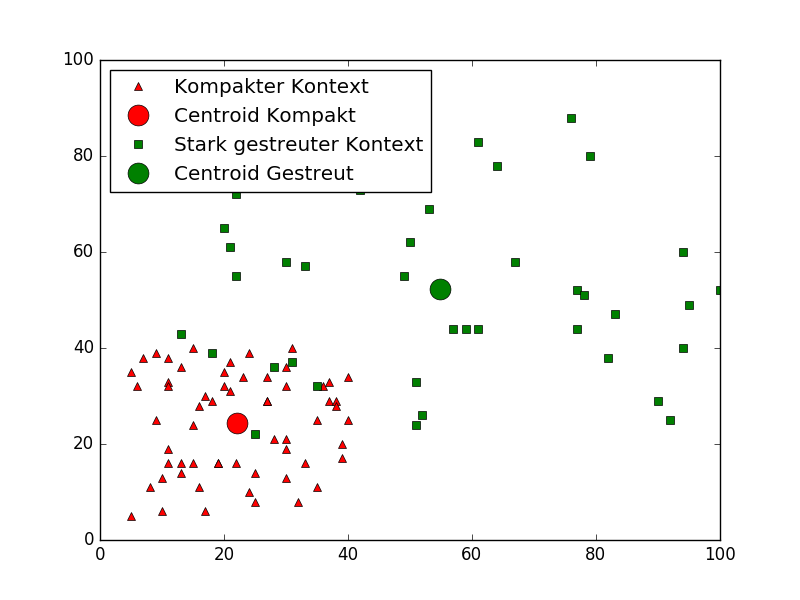
\includegraphics[width = \textwidth]{kontext}
    \caption{Streuung und Kompaktheit verschiedener Kontexte. Die beliebig dimensionalen Feature-Vektoren werden hier schematisch als Punkte im zweidimensionalen Raum dargestellt.}
    \label{kontext}
\end{figure}

Ein geeignetes Maß für die Kompaktheit des Kontextes zu finden, ist also entscheidend. Hierbei lässt sich ausnutzen, dass die Menge an Feature-Vektoren, die über den Kontext eines Wortes festgelegt wird, die Form eines \emph{Clusters} annimmt. In der Literatur finden sich einige Ansätze zur Evaluierung von verschiedenen Cluster-algorithmen (\citet{dunn1974}, \citet{Halkidi2001}). Für dieses Problem sind besonders Maße für die Kompaktheit eines einzelnen Clusters interessant, ohne dabei andere Cluster zu berücksichtigen. Ich möchte also für zwei zu vergleichende Wörter nicht wissen, wie gut ihre Kontexte in Cluster aufgeteilt wurden oder wie sehr die Cluster überlappen (obwohl das sicher auch einige interessante Informationen über die statistischen Eigenschaften der Kontexte liefern würde), sondern evaluieren, wie dicht oder kompakt die jeweiligen Cluster sind. Das Maß soll dann möglichst vom verwendeten Feature-raum abstrahieren und die Kompaktheit von Clustern über verschiedenen Vektorräume miteinander vergleichbar machen.

Ein Konzept, das aus der Cluster-evaluierung nutzbar gemacht werden kann, ist der \emph{Centroid} bzw. geometrische Schwerpunkt, der den Mittelpunkt aller Feature-Vektoren repräsentiert. Wie weit sind die einzelnen Feature-Vektoren vom Schwerpunkt entfernt? Hohe Distanz lässt auf eine weite Streuung schließen, niedrige Distanz auf Kompaktheit (vgl. Abbildung 1). Um das Maß nicht allzu sehr zu verkomplizieren, habe ich zur Bestimmung der Verteilung der Distanz der einzelnen Feature-Vektoren zum Schwerpunkt den Durchschnitt aller Distanzen gewählt.

Das vorgeschlagene dritte Maß für die semantische Spezifität eines Begriffes berechnet sich also wie folgt:

\begin{defi}
Seien $X_i$ die Menge aller Feature-Vektoren derjenigen Wörter, mit denen das Wort $w_i$ in einer Kontextrelation steht (s.o.), und $c_i$ der geometrische Schwerpunkt von $X_i$. \\ Dann ist der \textbf{Mean Distance to Centroid Score}

\begin{equation}
   mdcs_i =  \frac{1}{|X_i|} \sum_{x_j \in X_i} dist(x_j, c_i).
\end{equation}
\end{defi}

Die Menge der Wörter des Kontextes werden bei diesem Maß durch jeden von Null verschiedenen Wert im Feature-Vektor des Fokuswortes bestimmt. Um dem Umstand Rechnung zu tragen, dass die Kookkurrenz des Fokuswortes mit jedem Wort des Kontextes unterschiedlich ausgeprägt ist, verwende ich zusätzlich ein abgewandeltes Maß, das den kompletten Feature-Vektor des Kontextwortes mit der Ausprägung des zugehörigen Eintrags im Feature-Vektor des Fokuswortes skaliert.

\begin{defi}
Seien $X_i$ die Menge aller Feature-Vektoren derjenigen Wörter, mit denen das Wort $w_i$ in einer Kontextrelation steht (s.o.), $c_i$ der geometrische Schwerpunkt von $X_i$ und $a_{ij}$ der Eintrag des Feature-Vektors von Wort $w_i$ von Kontextwort $w_j$. \\ Dann ist der \textbf{Scaled Mean Distance to Centroid Score}

$$
  sca\_mdcs_i =  \frac{1}{|X_i|} \sum_{x_j \in X_i}  a_{ij} dist(x_j, c_i).
$$

\end{defi}

Damit ist $mdcs$ also nur ein Spezialfall von $sca\_mdcs$ mit $a_{ij} = 1$ für alle $i,j$.

Ein Ziel dieses Maßes ist es, das Resultat unabhängiger vom verwendeten Korpus zu machen. Ein Beispiel zur Verdeutlichung: Ein Korpus enthält ein Wort mit einer bestimmten \emph{Document Frequency}. Nun werden dem Korpus eine Menge von Texten hinzugefügt, die jedoch völlig andere Themengebieten behandeln und das Fokuswort nicht enthalten. Die \emph{Document Frequency} nimmt in starkem Maße ab. Angenommen, der Kontext des Wortes ist auch nicht sonderlich stark in den hinzugefügten Texten vertreten, dann steigt die \emph{Mean Distance to Centroid} nicht oder nicht signifikant.

\section{Semantische Spezifität: Experiment}

\subsection{Textgrundlage}

Ich verwende für dieses Experiment den Brown Corpus \citep{francis1979brown}, der eine repräsentative Momentaufnahme des englischen geschriebenen Sprachgebrauchs aus den 1960er Jahren mit etwa einer Millionen Token darstellt.

Die Wörter werden dabei allein durch lexikalische Erscheinungsform analysiert, es findet der Einfachheit halber \emph{keine} Bigram-analyse statt. Die Wörter werden dabei mittels Porter-Stemmer Algorithmus \citep{Porter:1997:ASS:275537.275705} auf ihre Grundform reduziert. Anschließend werden die Wörter über diese lexikalische Grundform identifiziert.

Zusätzlich schließe ich Wörter von der Analyse aus, die weniger als zehn Mal im Korpus auftreten, um zumindest etwas die Aussagekraft der statistischen Eigenschaften sicher zu stellen.

\subsection{Getestete Maße}

Im Experiment kombiniere ich die vorgestellten Maße miteinander. Zur Referenz liste ich hier alle relevanten getesteten Maße zur semantischen Spezifität. In der letzten Spalte der Tabelle steht die maximal erreichte Präzision. Für eine genaue Beschreibung siehe Abschnitt \ref{aufbau}.
\\\\
\textbf{Kookkurrenzmaße}:
\begin{itemize}
    \item Binär (Abschnit \ref{bin})
    \item Frequenz (Abschnitt \ref{freq})
    \item Dice-Koeffizient (Abschnitt \ref{dice}
    \item Chi Square (Abschnitt \ref{chi})
\end{itemize}

\noindent\textbf{Maße zur semantischen Spezifität (Scores)}:
\begin{itemize}
    \item Document Frequency (df, Abschnitt \ref{df})
    \item Non-Zero Dimensions (nzd, Abschnitt \ref{nzds})
    \item Mean Distance to Centroid (mdc, Abschnitt \ref{mdcs})
\end{itemize}

\noindent\textbf{Distanzmaße}:
\begin{itemize}
    \item standardisierte Euklidische Distanz  (Abschnitt \ref{eucl})
    \item Kosinusdistanz (Abschnitt \ref{cosi})
\end{itemize}

\begin{table}[h]
    \begin{center}
        \begin{tabular}{ l | l | l | l | l | r}
        Kontext   & K.-Maß    & Score         & Distanzmaß    & Kürzel            & Präzision \\ \hline \hline
        -               & -                 & dfs            & -             & df                        & 0.79 \\
        Satz            & -                 & nzds          & -             & nzds                 & 0.77 \\
        Satz            & Dice              & mdcs          & Kosinus       & dice\_mdcs\_cosi          & 0.74 \\
        Satz            & Dice              & mdcs          & Euklidisch    & dice\_mdcs\_eucl         & 0.79 \\
        Satz            & Frequenz          & mdcs          & Kosinus       & dice\_mdcs\_cosi          & 0.45 \\
        Satz            & Frequenz          & mdcs          & Euklidisch    & dice\_mdcs\_eucl          & 0.22 \\
        Fenster         & -                 & nzds          & -             & nzds                  & 0.80 \\
        Fenster         & Binär             & mdcs          & Kosinus       & bin\_mdcs\_cosi      & \textbf{0.81} \\
        Fenster         & Binär             & mdcs          & S-Euklidisch    & bin\_mdcs\_seuc      & 0.79 \\        
        Fenster         & Frequenz          & mdcs          & Kosinus       & freq\_mdcs\_cosi     & \textbf{0.83} \\
        Fenster         & Frequenz          & mdcs          & S-Euklidisch    & freq\_mdcs\_seuc     & 0.80 \\
        Fenster         & Frequenz          & scaled mdcs   & S-Euklidisch    & freq\_sca\_mdcs\_seuc & 0.79 \\
        Fenster         & Dice              & mdcs          & Kosinus       & dice\_mdcs\_cosi           & \textbf{0.81} \\
        Fenster         & Chi Square        & mdcs          & Kosinus       & chi\_mdcs\_cosi            & \textbf{0.82}
        \end{tabular}
    \end{center}
\end{table}

\subsection{Aufbau des Experiments} \label{aufbau}

Um die Validität der dargestellten Maße bewerten zu können, verwende ich eine Menge von Wortpaaren, bei denen offensichtlich ist, welches Wort die höhere semantische Spezifität besitzt. Sehr gute Kandidaten für diese Wortpaare sind Oberbegriffe und Unterbegriffe, also Begriffe, die andere Begriffe klassifizieren oder subsumieren. Diese Relation zwischen Begriffen impliziert, dass der Oberbegriff genereller und der Unterbegriff spezifischer ist. Die Liste der verwendeten Wortpaare ist \citet{Caraballo99determiningthe} entnommen und findet sich im Anhang.

Die verschiedenen Maße berechne ich nun zu jedem Wort der Wortpaare und vergleiche anschließend, welchen Begriff das Maß als semantisch spezifischer einstuft. Entspricht die Einstufung der Vorannahme, das der Unterbegriff semantisch spezifischer ist, wird das als richtige Einstufung gewertet. Die Präzision eines Maßes ist dann einfach der Anteil an geprüften Wortpaaren, den das Maß gemäß der Vorannahme richtig einstuft.

Von besonderem Interesse im Falle der Kontextfenster ist dabei die Größe des Kontextfensters. \citet[S. 68]{sahlgren2006word} findet in seinen Experimenten ein optimales Kontextfenster von der Größe 2+2, also zwei Wörter zu jeder Seite des Kontextwortes. Jedoch verweist er auch auf \citet{Miller2000-MILLRF}, die betonen, dass unser Verständnis von adäquaten Kontexten noch nicht perfekt ist und man nicht von vornherein ausschließen sollte, dass sich Kontexte auch anders verstehen lassen. Ausgehend von diesem Ansatz stelle ich die Resultate als Funktion der Größe des Kontextfensters dar (s. Abbildungen 3, 4 und 5.) und gehe ohne theoretische Vorannahmen an diese Fragestellung heran.

\subsection{Resultate}

\begin{figure}
    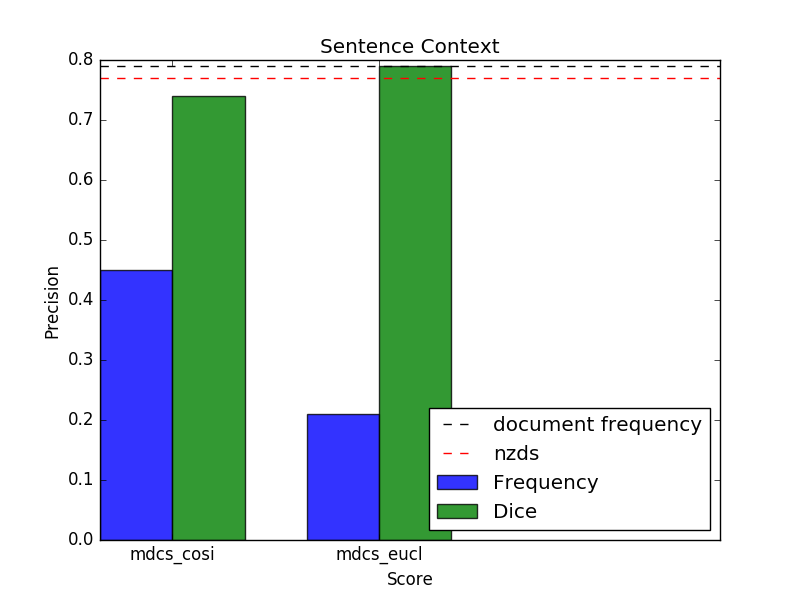
\includegraphics[width = \textwidth]{sent}
    \caption{Präzision der Maße mit Frequenz und Dice-Koeffizient im Satzkontext.}
    \label{sent}
\end{figure}
\begin{figure}
    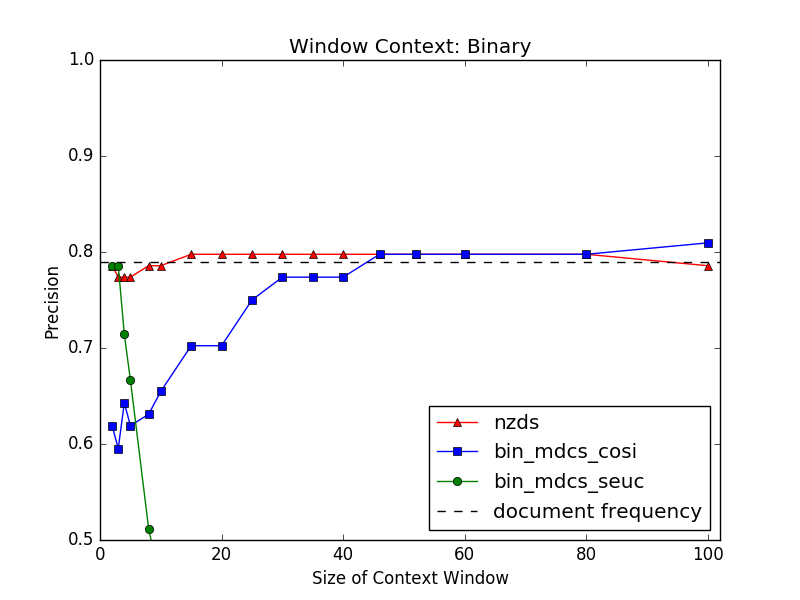
\includegraphics[width = \textwidth]{win_bin}
    \caption{Präzision der Maße mit binärem Kookkurrenzmaß im Fensterkontext über Größe des Fensterkontextes.}
    \label{win_bin}
\end{figure}
\begin{figure}
    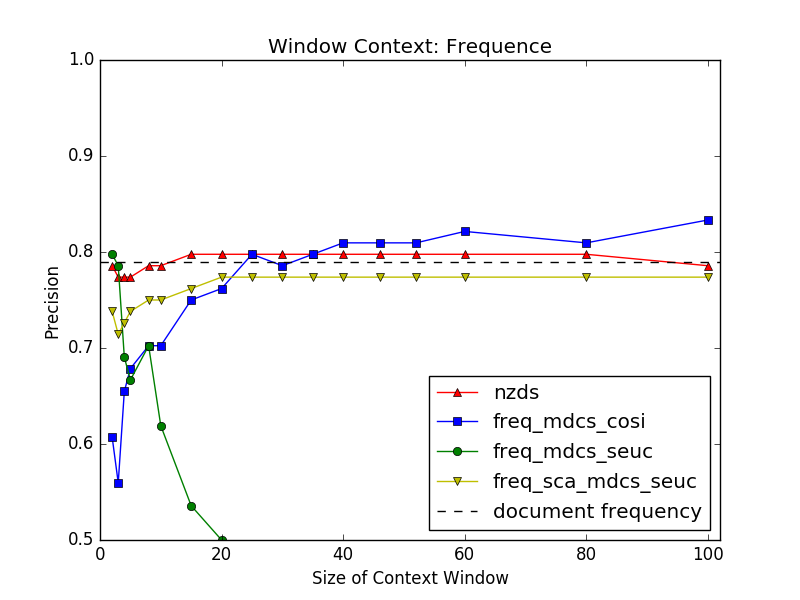
\includegraphics[width = \textwidth]{win_freq}
    \caption{Präzision der Maße mit Frequency Kookkurrenzmaß im Fensterkontext über Größe des Fensterkontextes.}
    \label{win_freq}
\end{figure}
\begin{figure}
    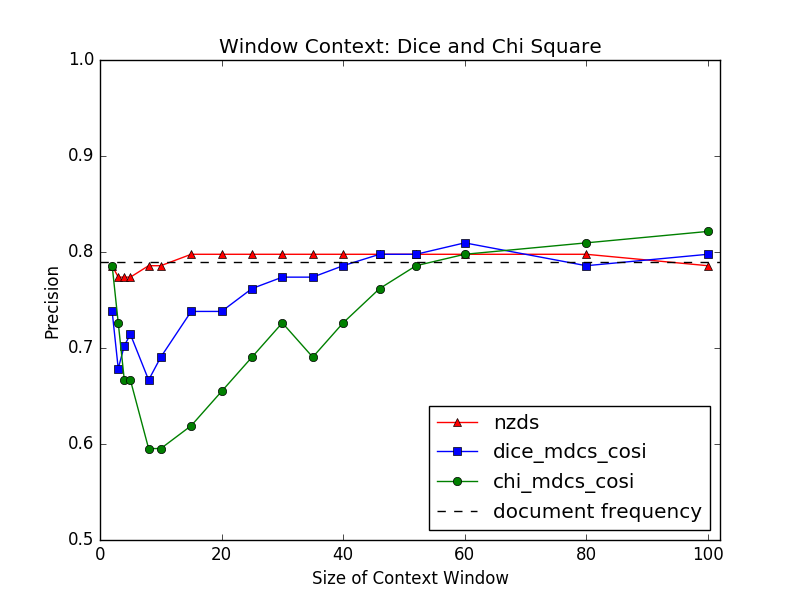
\includegraphics[width = \textwidth]{win_dice_chi}
    \caption{Präzision der Maße mit Dice bzw. Chi Square Kookkurrenzmaß im Fensterkontext über Größe des Fensterkontextes.}
    \label{win_dice_chi}
\end{figure}
Für alle Kontextfenstergrößen ist die \emph{Document Frequency} offensichtlich konstant. Zum Vergleich habe ich sie als gestrichelte Linie in jedes Diagramm eingezeichnet.

Der \emph{Non Zero Dimensions Score} ist weiterhin für jedes Kookkurrenzmaß identisch. Zum besseren Vergleich habe ich diesen Score auch in jedes Diagramm eingezeichnet (rot).

Der \emph{ndzs} ist dabei weitestgehend ähnlich präzise wie der \emph{dfs}, mit kleineren Schwankungen abhängig von der Fenstergröße.

\subsubsection {Satzkontext}

Die Ergebnisse der Analyse nach Satzkontext ist ernüchternd (siehe Abbildung \ref{sent}). Weder \emph{nzds} noch \emph{mcds} mit Kosinusmaß und standardisierter euklidischer Distanz erreichen die Präzisionswerte des Vergleichswert \emph{dfs}. Lediglich der Rückschritt auf einfache euklidische Distanz kann an die Vergleichswerte heranreichen. Dann jedoch gibt man die Vergleichbarkeit über verschiedene Vektorräume auf.


\subsubsection{Fensterkontext, Binäres}

Bemerkenswert ist hier, dass sich \emph{mdcs} mit Kosinusmaß und \emph{mdcs} mit euklidischer Distanz völlig unterschiedlich verhalten (siehe Abbildung \ref{win_bin}): Die Präzision bei Kosinusdistanz nimmt mit steigendem Kontextfenstergröße zu, die Präzision der euklidischen Distanz nimmt rapide ab. Interessanterweise ist die Präzision nur bei Kontextgröße $>80$ wirklich besser als der Vergleichswert \emph{dfs}.


\subsubsection{Fensterkontext, Frequency}

Es ergibt sich ein ähnliches Bild zum binären Maß (siehe Abbildung \ref{win_freq}). Auffällig ist jedoch, dass etwas früher, bei Fenstergröße 60, der \emph{mdcs} mit Kosinusdistanz ein klar besseres Ergebnis als der Vergleichswert liefert. Der skalierte \emph{mdcs} erreicht bei keiner getesteten Fenster den Vergleichswert.

\subsubsection{Fensterkontext, Dice Koeffizient und Chi Square}

Auch hier zeigt sich der für sehr kleine Fenstergrößen akzeptable Präzisionswert und das ausgeprägte Tief im Bereich $<30$ (siehe Abbildung \ref{win_dice_chi}). Auch auffällig, dass erst bei sehr großem Fensterkontext die Maße eine geeignete Präzision erreichen.


\subsection{Evaluation}

Sehr überraschend ist bei diesen Ergebnissen, dass sich mit einigen Scores bessere Resultate mit sehr großen Kontextfenstern erreichen lassen. Zunächst bestand die Befürchtung, dass kein Maß an die Präzision der simplen Heuristik der \emph{Document Frequency} herankommt. Die Ergebnisse zeigen allerdings, dass der hier vorgestellt Ansatz zumindest Potential hat, semantische Spezifität numerisch besser zu fassen als der $dfs$. In der sehr starken Simplifizierung in den Vorannahmen sind noch einige Verbesserungsmöglichkeiten enthalten, ebenso in der Auswertung der Ergebnisse, mehr dazu in Kapitel \ref{ausblick}.
Interessant auch, dass sich die Ergebnisse mit \citet[S. 35]{sahlgren2006word} decken, der das Kosinusmaß für am besten geeignet hält. Alle hier vorgestellten Scores auf Basis einer Wortraumdistanz zeigen die höchste Präzision bei Verwendung des Kosinusmaßes.

% \newpage
\section{Anwendung: Anglizismen}

Die Anwendung der vorgestellten performanten Maße auf vergleichende Anglizismen ist nun recht einfach: Wieder werden Wortpaare gebildet aus dem englischen Wort und seiner deutschen Entsprechung. Das Maß für das englische Fokuswort wird dann mittels englischem Korpus berechnet, das deutsche Fokuswort entsprechend mittels Deutschem. Die These, dass Anglizismen im Deutschen eine höhere semantische Spezifität aufweisen, lässt sich also experimentell bestätigen, wenn die Maße des englischen Fokusworts in der Regel höher als die des Deutschen ausfallen.

\subsection{Textgrundlage}

Um eine vergleichbare Textgrundlage im Deutschen wie Englischen zu verwenden, habe ich im Englischen auf den Reuters Corpus \citep{Lewis:2004:RNB:1005332.1005345} zurückgegriffen. Der Korpus umfasst in der verwendeten Version etwa 11.000 Nachrichtenartikel aus den späten 90ern.

Im Deutschen habe ich den Tiger Korpus \citep{Brants2004} verwendet, der eine vergleichbare Textmenge von Artikeln aus der Frankfurter Rundschau enthält.

Die verwendete Tokenisierung und das Stemming entspricht dem vorhergehenden Experiment. Die verwendete Liste von Anglizismen findet sich im Anhang. Von dieser Liste wurden nur solche verwendet, die öfter als zehnmal im Korpus auftraten. Die resultierende Liste findet sich im nächsten Abschnitt.

\subsection{Resultate}

Tabellen 1-4 zeigen die Resultate der präzisesten Maße aus dem vorhergehenden Experiment im Fensterkontext.

Da der vorliegende Tiger-Korpus keine Dokumentstruktur aufweist, wurde für dieses Experiment nicht der $dfs$ berechnet. Der $nzds$ zeigt jedoch zuverlässig sehr ähnliche oder bessere Präzision und wird in diesem Experiment als Benchmark verwendet.

Die Tabelle geben jeweils an, ob für den jeweiligen Anglizismus die Hypothese bestätigt wird, dass das englische Wort allgemeiner verwendet wird als das Deutsche (\emph{True / False}), d.h. ob der jeweilige Score des englischen Wortes höher ist als der des Deutschen.

\begin{table}[h]
    \begin{center}
        \begin{tabular}{ l | *{5}{c}  }
            Kookkurrenzmaß & - & binary & freq & chi\_sq & dice \\ \hline
               -      & nzds   &  mdcs\_cosi & mdcs\_cosi & mdcs\_cosi & mdcs\_cosi  \\ \hline
            Bar      &  \textbf{True}   &  False     &   False   &  \textbf{True}  & False    \\
            Bits     &  \textbf{True}   &  False     &   False   &  \textbf{True}   & False    \\
            Boom     &  \textbf{True}   &  False     &   False   &  \textbf{False}   & False    \\
            Date     &  \textbf{True}   &  False     &   False   &  \textbf{True}   & False   \\
            Image    &  \textbf{True}   &  False     &   True   &  \textbf{False}   & False   \\
            Manager  &  \textbf{True}   &  False     &   False   &  \textbf{True}   & True  \\
            Marketing&  \textbf{True}   &  False     &   False   &  \textbf{True}   & True   \\
            Service  &  \textbf{True}   &  False     &   False   &  \textbf{True}   & True   \\
            Star     &  \textbf{True}   &  False     &   False   &  \textbf{True}   & False  \\
            Test     &  \textbf{True}   &  False     &   False   &  \textbf{True} & False
        \end{tabular}
    \end{center}
    \caption{Fenstergröße 4}
\end{table}

\begin{table}[h]
    \begin{center}
        \begin{tabular}{ l | *{5}{c}  }
            Kookkurrenzmaß & - & binary & freq & chi\_sq & dice \\ \hline
               -      & nzds   &  mdcs\_cosi & mdcs\_cosi & mdcs\_cosi & mdcs\_cosi  \\ \hline
            Bar      &  \textbf{True}   &  False     &   False   &  \textbf{False}  & False    \\
            Bits     &  \textbf{True}   &  False     &   False   &  \textbf{True}   & False    \\
            Boom     &  \textbf{True}   &  False     &   False   &  \textbf{True}   & False    \\
            Date     &  \textbf{True}   &  False     &   False   &  \textbf{True}   & True   \\
            Image    &  \textbf{True}   &  False     &   False   &  \textbf{False}  & False   \\
            Manager  &  \textbf{True}   &  False     &   False   &  \textbf{True}   & True  \\
            Marketing&  \textbf{True}   &  True      &   True    &  \textbf{True}   & True   \\
            Service  &  \textbf{True}   &  False     &   False   &  \textbf{True}   & True   \\
            Star     &  \textbf{True}   &  False     &   False   &  \textbf{True}   & False  \\
            Test     &  \textbf{True}   &  False     &   False   &  \textbf{True}  & True
        \end{tabular}
    \end{center}
    \caption{Fenstergröße 25}
\end{table}

\begin{table}[h]
    \begin{center}
        \begin{tabular}{ l | *{5}{c}  }
            Kookkurrenzmaß & - & binary & freq & chi\_sq & dice \\ \hline
               -      & nzds   &  mdcs\_cosi & mdcs\_cosi & mdcs\_cosi & mdcs\_cosi  \\ \hline
            Bar      &  \textbf{True}   &  False     &   False   &  \textbf{True}  & False    \\
            Bits     &  \textbf{True}   &  False     &   False   &  \textbf{True}   & False    \\
            Boom     &  \textbf{True}   &  False     &   False   &  \textbf{True}   & False    \\
            Date     &  \textbf{True}   &  False     &   False   &  \textbf{True}   & True   \\
            Image    &  \textbf{False}  &  False     &   False   &  \textbf{False}  & False   \\
            Manager  &  \textbf{True}   &  False     &   False   &  \textbf{True}   & True  \\
            Marketing&  \textbf{True}   &  True      &   True    &  \textbf{True}   & True   \\
            Service  &  \textbf{True}   &  False     &   False   &  \textbf{True}   & True   \\
            Star     &  \textbf{True}   &  False     &   False   &  \textbf{True}   & False  \\
            Test     &  \textbf{True}   &  False     &   False   &  \textbf{True}  & True
        \end{tabular}
    \end{center}
    \caption{Fentergröße 60}
\end{table}

\begin{table}[h]
    \begin{center}
        \begin{tabular}{ l | *{5}{c}  }
            Kookkurrenzmaß & - & binary & freq & chi\_sq & dice \\ \hline
               -      & nzds   &  mdcs\_cosi & mdcs\_cosi & mdcs\_cosi & mdcs\_cosi  \\ \hline
            Bar      &  \textbf{True}   &  False     &   False   &  \textbf{True}   & False    \\
            Bits     &  \textbf{True}   &  False     &   False   &  \textbf{True}   & False    \\
            Boom     &  \textbf{True}   &  False     &   False   &  \textbf{True}   & False    \\
            Date     &  \textbf{True}   &  False     &   False   &  \textbf{True}   & True   \\
            Image    &  \textbf{False}  &  False     &   False   &  \textbf{True}   & False   \\
            Manager  &  \textbf{True}   &  False     &   False   &  \textbf{True}   & True  \\
            Marketing&  \textbf{True}   &  True      &   True    &  \textbf{True}   & True   \\
            Service  &  \textbf{True}   &  True      &   False   &  \textbf{True}   & True   \\
            Star     &  \textbf{True}   &  False     &   False   &  \textbf{True}   & False  \\
            Test     &  \textbf{True}   &  False     &   False   &  \textbf{True}   & True
        \end{tabular}
    \end{center}
    \caption{Fentergröße 100}
\end{table}

\subsection{Evaluation}

Die Resultate dieses Experiments sind überraschend uneindeutig, gegeben die eher einheitlichen Ergebnisse aus dem vorangegangenen Experiment. Eigentlich würde man erwarten, dass sich die Scores relativ einig sind, was die höhere Spezifität der Worte angeht. Die Ergebnisse sind jedoch gemischt: Während der $ndzs$ fast ausschließlich die Hypothese bestätigt, schwanken die anderen Maße sehr stark in der Ausprägung. Gegeben, dass die Maße für einen einheitlichen Korpus alle relativ zuverlässig sind, lässt das nun zwei verschiedene Erklärungen zu:

\begin{enumerate}
    \item Die Hypothese ist falsch: Es ist nicht der Fall, dass Anglizismen dazu tendieren, semantisch spezifischer zu sein als ihr englisches Ursprungswort.
    \item Die Vergleichsmaße über verschiedene Korpora sind nicht so unabhängig vom Korpus, wie ich erwartet habe.
\end{enumerate}
Ich tendiere stark dazu, Erklärung 2 anzunehmen. Die Einheitlichkeit der Ergebnisse über verschiedene Korpora hinweg wurde noch nicht experimentell bestätigt. Das wäre definitiv wünschenswert, würde aber leider den Rahmen der vorliegenden Arbeit vollends sprengen. Beim Vergleich der Korpora fällt stark die unterschiedliche Dimensionierung auf: Englischer Korpus (Reuters): 4847 Wörter nach Normalisierung. Deutscher Korpus (Tiger): 6179 Wörter nach Normalisierung. Bei Reduzierung der Dimensionen auf 4951 durch Erhöhung des Frequency-Thresholds im Tigerkorpus auf 13 (statt 10) sind die erzielten Ergebnisse sehr viel eindeutiger und alle verwendeten Maße tendieren dazu, das englische Wort als genereller auszuzeichnen. Dies legt den Schluss nahe, dass die Hypothese zwar richtig ist, die verwendeten Maße jedoch nicht so unabhängig vom verwendeten Korpus sind wie gewünscht. Lediglich der $nzds$ und $chi\_mdcs\_cosi$ scheinen hier nicht so anfällig zu sein. Die Bestätigung der Robustheit der Maße steht also noch aus. Insbesondere wäre es interessant zu sehen, \emph{warum} sich diese Maße unterschiedlich verhalten. Für eine tiefer gehende Analyse ist leider in dieser Arbeit kein Platz.

\section{Konklusion}

Im ersten Teil des Experiments konnte die von \citet{Caraballo99determiningthe} gefundene Performanz der \emph{Document Frequency} bestätigt werden. Unter den neu formulierten Maßen wurden einige gefunden, die in einer festen Textmenge Wörter mit höherer Zuverlässigkeit als spezieller auszeichnen können, als es die \emph{Document Frequency} kann. Das kann man als kleinen Erfolg werten, der die aufgestellten Hypothesen (s. Einleitung) über den Zusammenhang von Spezifität und Kontext eines Wortes bestätigt.

Problematischer wird es beim Vergleich unterschiedlicher Korpora und unterschiedlicher Sprachen. Die experimentelle Bestätigung der Validität der Maße steht noch aus (s. nächster Abschnitt), allerdings besteht die berechtigte Hoffnung, das auch über verschiedene unangeglichene Korpora hinweg verlässlich das generellere Wort bestimmt werden kann. Insbesondere der \emph{Non-Zero Dimensions Score} und der \emph{Chi Square Mean Distance to Centroid Cosine Score} sind dabei vielversprechend.

Die These, dass Anglizismen im Deutschen semantisch spezifischer sind als ihre englischen Ursprungswörter, wurde in diesem Experiment also nicht eindeutig bestätigt, jedoch sehe ich Grund zur Annahme, dass durch Auswahl und Test angemessener Maße bessere Ergebnisse erzielt werden können.

\section{Caveats und Ausblick} \label{ausblick}

Die vorgestellt Auswertung ist vergleichsweise makroskopisch und soll einen Überblick über die Tauglichkeit verschiedener Verfahren liefern. Die Analyse einzelner Maße kann allerdings auch sehr aufschlussreich sein: So kann man sich etwa die Berechnungen einzelner Wortpaare genauer anschauen und so Schwachstellen oder Stärken des jeweiligen Maßes herausfinden.

Ein großer Vorteil der vorgestellten Maße ist, dass sie völlig generell und nicht themenbezogen sind, und zusätzlich ohne Trainingsdaten auskommen. Andere Verfahren, etwa über Klassifizierer, könnten allerdings performanter sein.

Ein Aspekt, der in dieser Arbeit nicht berücksichtigt wurde, ist die Gewichtung der Kookkurrenzen nach Distanz zum Fokuswort. Hier wurden alle Wörter, die im Kontextfenster auftauchen, gleich gewichtet, um die Maße nicht noch mehr zu verkomplizieren. Diese Änderung könnte bewirken, dass die signifikanten Kookkurrenzen noch mehr im Vordergrund stehen.

Ich habe hier vorausgesetzt, dass die getesteten Maße auch in anderen Kontexten und Sprachen (etwa im Deutschen) greifen. Das habe ich zwar grob getestet, aber keinem rigorosen Text unterzogen. Diese Hilfshypothesen erfordern eigentlich auch noch einiges an experimenteller Bestätigung. Zwar habe ich auch in einem ersten Test überprüft, ob die Maße im Deutschen richtige Ergebnisse liefern (die Präzision der verschiedenen Maße ähnelt sich stark), eine experimentelle Bestätigung der Vergleichbarkeit der Maße aus einem Korpus mit denen eines anderen steht noch aus. Insbesondere verschiedene Verhältnisse der Korpora zueinander sollten hier Testparameter sein. Wie verhalten sich die Maße bei Korpora aus unterschiedlichen Themengebieten? Wie bei stark unterschiedlicher Größe?

Die hier vorgestellte Methode und das anschließende Experiment beinhalten einige vereinfachende Vorannahmen, die das Endergebnis negativ beeinflussen könnten. Ein großer Faktor ist wahrscheinlich, dass Wörter allein aufgrund ihrer lexikalischen Form identifiziert wurden. Es ist natürlich bekannt, dass gleiche lexikalische Formen unterschiedliche Bedeutungen tragen können, also ambig sind. Das hat direkten Einfluss auf den Feature-Vektor des Wortes - so werden auch alle Kookkurrenzen dazu gezählt, die eigentlich einer anderen Wortbedeutung zugerechnet werden sollen. Abhilfe kann hier eine \emph{Word Sense Disambiguierung} schaffen, bei der in der Präprozessierung oder bereits vorher, mittels eines annotierten Korpus, die verschiedenen Wortbedeutungen auseinandergehalten werden.

Auch wurde keinerlei Unterscheidung gemacht hinsichtlich der Art des untersuchten Wortes und seiner Beziehung zu den umliegenden Wörtern, außer die direkte lexikalische Nachbarschaft. So wurden z.B. nicht Nomen untersucht und der Kontext aus Verben gebildet, die in direkter Subjekt-Prädikat-Relation stehen. Eine solche tiefer gehende Analyse könnte u.U. dazu beitragen, die Erkennung von semantischer Spezifität zu präzisieren.

Ein weiteres interessantes Maß wird in \citet{Sahlgren2005} beschrieben. Dieses Maß ist dafür vorgesehen zu bestimmen, wie dicht (\emph{dense}) ein Wortraum ist, d.h. wie kompakt oder gestreut der Wortraum mit Einträgen gefüllt ist. Die Ergebnisse werden dann dazu verwendet, verschiedene Korpora dahingehend zu vergleichen, wie thematisch ähnlich sie sich sind. Dazu werden zu jedem Punkt des Raumes die zehn nächsten Nachbarn bestimmt, dann wiederum die zehn nächsten Nachbarn. Der Durchschnitt der Anzahl der so gesammelten unique Worte bildet das Maß; es reicht von zehn (maximale Dichte) bis 100 (maximale Streuung). Dieser Ansatz scheint sehr gut auch auf semantische Spezifität zu passen und die Dichte eines Kontextes darstellen zu können. Um es noch unabhängiger vom verwendeten Korpus zu machen und so auch auf das Problem der Anglizismen anwenden zu können, kann man das Verhältnis vom Maß des Kontextes zum Maß des ganzen Korpus verwenden und hat so ein Maß von $0,1$ (maximale Dichte) bis $1,0$ (maximale Streuung). Ein interessanter Ansatz, der es leider nicht mehr in die Arbeit geschafft hat.

Die Auswertung der Resultate ist in der vorliegenden Form eher simplistisch. So wird einfach nur verglichen, welches Maß den höheren Wert berechnet hat und dann auf höhere bzw. niedrigere semantische Spezifität geschlossen. Was eigentlich gewünscht ist, wäre eine statistisch zuverlässige Aussage. Die Entscheidung über die Spezifität sollte mit einer gewissen Sicherheit erfolgen. Um das zu erreichen, müsste man zunächst über zufällig ausgewählte Samples aus dem Korpus eine generelle Verteilung der Differenzen der Spezifitätsmaße von Wortpaaren berechnen. Auf dieser Grundlage ließe sich die Standardabweichung der Differenz berechnen. Unter der Zusatzannahme, dass diese Differenz normal verteilt ist (was sich auch prüfen ließe), kann dann die statistische Signifikanz der Differenz der Maße eines Wortpaares berechnet werden, dessen semantische Spezifität man untersuchen will. So könnte dann etwa erst ab einem bestimmten Schwellenwert mit großer Sicherheit davon gesprochen werden, ob sich hier semantische Spezifität stark unterscheidet. Aber gleichzeitig wird auch die Präzision der Antwort erhöht, bei unzureichender Ausprägung enthält sich das Maß dann einer Wertung. Hat man auf diese Weise ein Maß für die Zuversicht in die Einschätzung des Maßes gefunden, lassen sich auch mehrere performante Scores aggregieren und so in einem Hybrid-Verfahren eine noch höhere Performanz erreichen. So kann bei widerstreitenden Ergebnissen zweier Maße dasjenige Maß mit der höheren Zuversicht entscheiden. Durch diese Aggregation entsteht dann ein neues, noch zuverlässigeres Verfahren.

\bibliography{spinfohausarbeit}

\section{Anhang}

\subsection{Wordpaare}

\begin{description}
    \item[food]beverage, dessert, bread, cheese, meat, dish, butter, cake, egg, candy, pastry, vegetable, fruit, sandwich, soup, pizza, salad, relish, olives, ketchup, cookie
    \item[beverage] alcohol, cola
    \item[alcohol] iquor, gin, rum, brandy, cognac, wine, champagner,
    \item[meat] liver, ham
    \item [dish] sandwich, soup, pizza, salad
    \item[vegetable] tomato, mushroom, legume
    \item[fruit] pineapple, apple, peaches, strawberry
    \item[vehicle] truck, car, trailer, campers
    \item[car] jeep, cab, coupe
    \item[person] worker, writer, intellectual, professional, leader, editor, entertainer, engineer,technician, journalist, commentator, novelist
    \item[intellectual] physicist, historian, chemist
    \item[professional] physician, educator, nurse, dentist
    \item[entity] organism, object
    \item[animal] mammal, bird, dof, car, horse, chicken, duck, fish, turtle, snake
    \item[mammal] cattle, dog, cat, horse
    \item[bird] chicken, duck
    \item[fish] herring, salmon, trout
    \item[metal] alloy, steel, gold, silver, iron
    \item[location] region, country, state, city
    \item[substance] food, metal, carcinogen, fluid
    \item[fluid] water
    \item[commodity] clothing, appliance
    \item[artifact] covering, paint, roof, curtain, decoration, drug
    \item[publication] book, article
    \item[fabric] wool, nylon, cotton
    \item[facility] airport, headquarters, station
    \item[structure] house, factory, store
    \item[organ] heart, lung
\end{description}
\subsection{Anglizismen}

Airline, Babysitter, Bachelor, Bar, Basketball, Beach, Beat, Bestseller, Bits, Blackout, Blues, Bodybuilder, Boom, Boss, Box, Boys, Braindrain, Browser, Camper, Campus, Champion, clever, Coach, Cola, Comedy, Container, cool, Copyright, Date, Deal, Design, Drinks, Foul, Freak, Gameshow, Gangster, Hattrick, Hit, Hooligans, Image, Insider, Internet, Jazz, Keeper, Kids, Leasing, Lifestyle, Lobby, mail, Manager, Marketing, Meeting, model, Performance, Pixel, Poker, Pool, Punk, Quiz, Radar, Rapper, Scanner, Service, shop, Skateboard, Soccer, Sponsor, Stalker, Star, Start-up, Stewardess, Striptease, Surfer, super, Test, Training, Tricks, unfair, Website, Yacht, Yankee

\subsection{Verwendete Technologien}

Das Experiment wurde komplett in \texttt{python 3.5.2} umgesetzt.

Den Zugang zu den Korpora habe ich mittels der Python-Bibliothek \texttt{nltk} realisiert. Auch die verwendeten Tokenisierer und Stemmer entstammen dieser Bibliothek. Die Berechnung der verschiedenen Kookkurrenzmaße erfolgten mit dieser Bibliothek.

Mathematische maschinennahe Berechnungen insbesondere für Matrizen habe ich mittels der Python-Bibliotheken 
\texttt{numpy} und \texttt{scipy} umgesetzt. Besonders bei der Berechnung der verschiedenen Distanzmaße waren diese Bibliotheken hilfreich.

Der Programmcode ist unter MIT License zugänglich unter \\ \texttt{https://github.com/conradfriedrich/termspec}.


\nocite{han2011}
\nocite{heyer2008}
\nocite{manning1999}


\newpage

Hiermit versichere ich an Eides statt, dass ich diese Arbeit selbstständig verfasst
und keine anderen als die angegebenen Quellen und Hilfsmittel benutzt habe.
Die Stellen meiner Arbeit, die dem Wortlaut oder dem Sinne nach anderen
Werken und Quellen, einschließlich Quellen aus dem Internet, entnommen sind,
habe ich in jedem Fall unter Angabe der Quelle deutlich als Entlehnung kenntlich
gemacht. Dasselbe gilt sinngemäß für Tabellen, Karten und Abbildungen. Diese
Arbeit habe ich in gleicher oder ähnlicher Form oder auszugsweise nicht im
Rahmen einer anderen Prüfung eingereicht.\\\\\\

\noindent\rule{8cm}{0.4pt}
(Unterschrift)


\end{document}